\newcommand{\siecle}[1]{\textsc{#1}\ieme}
\chapter{Le contexte théorique}
\label{chap.ms}
Au cours du \siecle{xx} siècle, les progrès dans la compréhension des phénomènes qui régissent les constituants élémentaires de la matière ont été très importants. Entre la découverte de l'électron par J.J Thomson en 1897 puis celle d'un boson compatible avec le boson de Higgs en 2012 au LHC (Large Hadron Collider), plusieurs découvertes et prédictions ont permis de mieux comprendre la structure de la matière et de construire la théorie sous-jacente: le modèle standard. Dans ce chapitre, nous présenterons les différents constituants de la matière et leur mécanismes d'interaction dans le cadre du modèle standard. Nous terminerons ce chapitre en présentant quelques limites de cette théorie.
\minitoc
\newpage

%%%%%%%%%%%%%%%%%%%%%%%%%%%%%%%%%%%%%%%%%%%%%%%

\section{Le modèle standard}
\begin{figure}[!ht]
  \begin{center}
    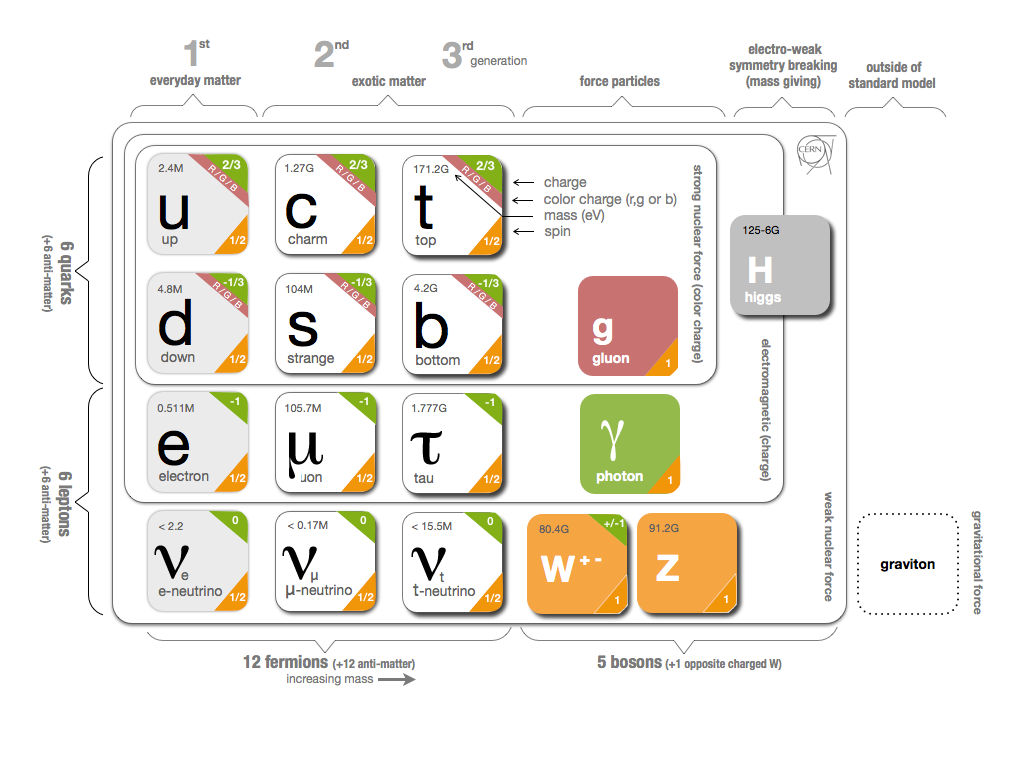
\includegraphics[width=.7\textwidth]{ModelStandard/figs/Standard_model_infographic_bis.png}
    \caption{Classification des quarks, des leptons et des bosons vecteurs.}
    \label{fig:mc}
  \end{center}
\end{figure}
Le modèle standard est une théorie de jauge basée sur le groupe de symétrie $SU(3)\times SU(2)\times U(1)$. Le groupe $U(1)$ permet de décrire l'électrodynamique quantique et le groupe $SU(2)$ l'interaction faible. Le groupe de symétrie $SU(2)\times U(1)$ permet de décrire l’interaction électrofaible. La chromodynamique quantique qui décrit les interactions fortes est basée sur le groupe $SU(3)$. Dans le modèle standard, les particules sont réparties en plusieurs familles. La figure~\ref{fig:mc} présente les différentes familles de particules dans le cadre du modèle standard. On trouve tout d'abord 12 fermions (particules de spin $1/2$) répartis en deux familles : les leptons et les quarks. Ces deux familles se divisent en trois générations de doublet de particules. Les premières générations de quarks et de leptons contiennent les particules les plus légères et constituent la matière stable de notre univers. Les particules plus massives des autres générations ont un temps de vie plus court et ne sont créées que dans des processus de haute énergie. A ces 12 fermions, il faut ajouter leur 12 antiparticules qui ont les mêmes masses mais des charges quantiques (charge électrique, saveur, couleur pour les quarks) opposées. Ces fermions interagissent entre eux grâce à l'échange de 4 bosons vecteurs (particules de spin entier). Un cinquième boson apparaît dans le mécanisme de Higgs, nécessaire pour introduire la masse des particules dans la théorie. 
\subsection{Les leptons}
Nous avons vu que trois générations de doublet constituent la famille des leptons. La première génération contient l'électron et le neutrino électronique. L'électron a été découvert à la fin du \siecle{xix} siècle. L'existence du neutrino électronique est postulée en 1930 pour respecter les lois de conservation de l'énergie, de l'impulsion et du spin dans la désintégration $\beta$ et confirmée en 1956 auprès de réacteurs nucléaires. Le muon, le tau et leurs neutrinos associés viennent compléter la famille des leptons. %Notons aussi la notion de saveur des leptons. On dénombre trois saveurrs pour les leptons: la saveur électronique, muonique et tauique. La saveur électronique vaut 1 pour les leptons de la première génération, 0 pour les leptons des deuxième et troisième génération et -1 pour les anti-leptons de la première génération. La saveur leptonique est un nombre quantique qui reste conservé dans la plupart des interactions. 
\begin{table}[!ht]
  \begin{center}
    \small
    \begin{tabular}{c|c|c|c}
      \rowcolor{black!20!white}Génération & Lepton & Masse & Charge électrique\\
      \rowcolor{black!5!white}\hline
      \rowcolor{black!5!white}$1$ & $e^-$ & $511~keV$ & $-1$ \\
      \rowcolor{black!5!white}$ $ & $\nu_e$ & $<2.2~eV$ & $0$ \\
      \rowcolor{black!5!white}\hline
      \rowcolor{black!5!white}$2$ & $\mu^-$ & $105.7~MeV$ & $-1$ \\
      \rowcolor{black!5!white}$ $ & $\nu_{\mu}$ & $<0.17~MeV$ & $0$ \\
      \rowcolor{black!5!white}\hline
      \rowcolor{black!5!white}$3$ & $\tau^-$ & $1776.8~MeV$ & $-1$ \\
      \rowcolor{black!5!white}$ $ & $\nu_{\tau}$ & $<15.5~MeV$ & $0$ \\
    \end{tabular}
  \end{center}  
  \caption{Propriétés des leptons du modèle standard. Les charges sont données en unité de charge élémentaire ($e=1.6\times10^{-19}~C$).}
  \label{tab.lepton_pro}
\end{table}
Le tableau~\ref{tab.lepton_pro} présente la masse et la charge des différents leptons des trois générations. Les neutrinos, n'étant pas chargés, n'interagissent qu'à travers l'interaction faible. Les autres leptons interagissent à travers les interactions faible et électromagnétique. Dans le modèle standard, les neutrinos sont prédits avec une masse nulle. Cependant, les expériences qui étudient l'oscillation des neutrinos semblent indiquer que la masse de ces particules n'est pas nulle. 

\subsection{Les quarks}
Les quarks ont été introduits pour expliquer la structure des hadrons comme les protons et les neutrons. Les quarks sont de spin $1/2$ et comme pour les leptons sont classés en trois générations de doublet. Les quarks $up$ ($u$) et $down$ ($d$) sont les quarks de la première génération. Ils sont les quarks les plus légers et sont les constituants des protons et des neutrons. La deuxième génération est constituée des quarks $charm$ ($c$) et $strange$ ($s$) et la troisième des quarks $bottom$ ($b$) et $top$ ($t$). Ces particules ont une charge fractionnaire de la charge élémentaire. Le tableau~\ref{tab.quark_pro} présente la masse et la charge des différents quarks des trois générations \cite{pdg}. 
\begin{table}[!ht]
  \begin{center}
    \begin{tabular}{c|c|c|c}
      \rowcolor{black!20!white}Génération & Quark & Masse & Charge électrique\\
      \rowcolor{black!5!white}\hline
      \rowcolor{black!5!white}$1$ & $u$ & $2.3^{+0.7}_{-0.5}~MeV$ & $+2/3$ \\
      \rowcolor{black!5!white}$ $ & $d$ & $4.8^{+0.5}_{-0.3}~MeV$ & $-1/3$ \\
      \rowcolor{black!5!white}\hline
      \rowcolor{black!5!white}$2$ & $c$ & $1.275\pm0.025~GeV$ & $+2/3$ \\
      \rowcolor{black!5!white}$ $ & $s$ & $95\pm5~MeV$ & $-1/3$ \\
      \rowcolor{black!5!white}\hline
      \rowcolor{black!5!white}$3$ & $t$ & $173.21\pm0.51\pm0.71~GeV$ & $+2/3$ \\
      \rowcolor{black!5!white}$ $ & $b$ & $4.18\pm0.03~GeV$ & $-1/3$ \\
    \end{tabular}
  \end{center}  
  \caption{Propriétés des quarks du modèle standard. Les charges sont données en unité de charge élémentaire ($e=1.6\times10^{-19}~C$). Seule la masse du quark $top$ provient d'une mesure directe. Les masses des autres quarks sont, à cause de leur confinement dans les hadrons, déterminées indirectement par leur influence sur la matière hadronique.}
  \label{tab.quark_pro}
\end{table}
Les quarks sont soumis aux interactions électromagnétique et faible comme pour les leptons, mais aussi à l'interaction forte. La chromodynamique quantique est la théorie qui décrit l'interaction forte. Cette théorie introduit un nouveau nombre quantique: la couleur. Ainsi, les quarks sont vert, bleu ou rouge et peuvent changer de couleur en interagissant fortement grâce à l'échange de gluons. Les anti-quarks sont de couleur anti-vert, anti-rouge ou anti-bleu. L'intensité de l'interaction forte augmente avec la distance entre les quarks. Ainsi les quarks sont confinés dans des hadrons. Les hadrons sont des particules composites, constituées de quarks ou d'anti-quarks et de gluons. On trouve deux familles de hadrons: les baryons composés de trois quarks ou trois anti-quarks, et les mésons composés d'un quark et d'un anti-quark. Les hadrons ont une charge de couleur nulle (ou blanche): les baryons ont donc un quark vert, un rouge et un bleu tandis que les mésons sont constitués d'un quark bleu et d'un anti-quark anti-bleu (ou rouge/anti-rouge, vert/anti-vert). Le confinement des quarks dans les hadrons est une propriété importante en physique des particules. En effet, lorsque deux quarks s'éloignent l'un de l'autre, l'énergie potentielle due à l'interaction forte augmente aussi. Si l'énergie est suffisante, une paire de quark et d'anti-quark peut être créée. Ce phénomène de multiplication donne des jets de hadrons après des collisions entre particules. Ce phénomène est aussi présent dans les premières interactions des particules avec la matière conduisant aux gerbes hadroniques (cf. chapitre~\ref{chap.shower}).

\subsection{Les bosons vecteurs et les interactions du modèle standard}
Dans le modèle standard, les différentes particules interagissent entre elles en s'échangeant un boson vecteur ou boson de jauge. 

Le photon est le boson vecteur échangé lors d'une interaction électromagnétique entre particules chargées. Le photon n'est pas chargé, de masse nulle et de spin 1. L'interaction électromagnétique est de portée infinie et son intensité varie comme $1/r^2$ (où $r$ est la distance entre les deux particules chargées).

L'interaction faible est portée par les bosons $Z$ ($m_Z=91.188\pm0.002~GeV$) et $W^\pm$ ($m_W=80.385\pm0.015~GeV$) \cite{pdg}. Cette interaction est responsable de la désintégration des particules. Elle a été introduite en 1930 pour expliquer la désintégration $\beta$ du neutron en proton. Ses bosons vecteurs étant massif, cette interaction est de courte portée ($\simeq10^{-17}~m$). L'interaction faible permet de modifier la saveur des quarks. La saveur des leptons reste conservée lors d'une réaction faible. La figure~\ref{fig:beta} montre un diagramme de Feynman illustrant la désintégration $\beta$ du neutron en proton. 
\begin{figure}[!ht]
  \begin{center}
    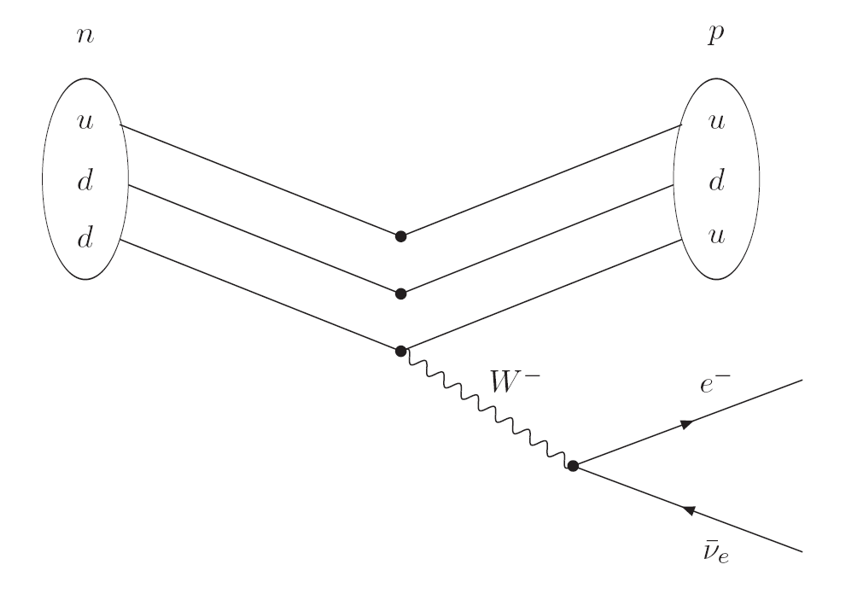
\includegraphics[width=.5\textwidth]{ModelStandard/figs/betaminus.png}
    \caption{Diagramme de Feynman associé à la désintégration $\beta$ du neutron en proton. Un quark $d$ du neutron change de saveur en quark $u$. L'interaction s'accompagne de l'émission d'un électron et d'un anti-neutrino électronique.}
    \label{fig:beta}
  \end{center}
\end{figure}
Le changement de saveur d'un quark $d$ en $u$ est accompagné par l'émission d'un électron et d'un neutrino électronique. 

Les interactions électromagnétique et faible ont été unifiées dans le modèle standard. On parle maintenant d’interaction électrofaible. Cependant, les bosons introduits dans le modèle électrofaible apparaissaient avec une masse nulle, ce qui était en contradiction avec les observations expérimentales. Ainsi, un mécanisme de brisure spontanée de la symétrie électrofaible a été introduit pour rétablir la masse des bosons $W^\pm$ et $Z$ (cf. section~\ref{sec.higgs}).

La dernière interaction du modèle standard est l'interaction forte. Elle est la force responsable de la cohésion des nucléons. Cette interaction est décrite par la chromodynamique quantique, basée sur le groupe de symétrie $SU(3)$. Ainsi, huit bosons vecteurs sont associés à cette interaction: les gluons. Ces bosons sont de masse nulle, de spin 1 et ne sont pas chargées. Comme pour les quarks, les gluons portent une charge de couleur et peuvent donc interagir fortement entre eux. La masse nulle des gluons indique une portée infinie de l'interaction forte. Cependant le confinement des quarks limite la portée de cette interaction dans les hadrons. 

\section{Le mécanisme de Higgs}
\label{sec.higgs}
Le mécanisme de Higgs, ou plutôt de Brout-Englert-Higgs a été introduit en 1964 pour expliquer la masse des bosons de l'interaction électrofaible. Pour faire apparaître un terme de masse aux bosons de l'interaction électrofaible, il est nécessaire d'utiliser un mécanisme de brisure spontanée d'une symétrie de jauge locale. La symétrie est brisée en introduisant un champ scalaire avec une valeur moyenne non nulle dans le vide. Cette procédure introduit alors plusieurs champs, assimilés à des bosons dans la théorie:
\begin{itemize}
\item un champ scalaire réel massif : le boson de Higgs (de spin 0);
\item un champ vectoriel réel de masse nulle : le photon (de spin 1);
\item un champ vectoriel réel massif : le boson $Z$ (de spin 1);
\item un champ vectoriel complexe massif qui représente une paire particule-antiparticule : les bosons $W^\pm$ (de spin 1).
\end{itemize}
Dans ce modèle, les masses des fermions sont obtenues grâce au couplage de ces fermions au champ de Higgs. Les neutrinos n'interagissent pas avec ce champ et sont donc sans masse dans la théorie. 

Le mécanisme de Higgs permet donc d'expliquer la masse des particules du modèle standard. Cependant, ce mécanisme fait apparaître un nouveau boson massif de spin 0: le boson Higgs. En 2012, les expérience CMS et ATLAS auprès du collisionneur de hadron LHC ont annoncé avoir découvert une particule avec une masse comprise entre 125 et 127 $GeV$, compatible avec le boson de spin 0 de la théorie. Pour l'instant les mesures des différents couplages de cette particule aux autres particules semblent indiquer que cette particule est bien le boson de Higgs du modèle standard \cite{CMS-PAS-HIG-14-009}. Une propriété fondamentale au boson de Higgs reste cependant à observer. En effet, dans le modèle standard, le boson de Higgs interagit avec lui même. Une signature expérimentale de l'auto-couplage du boson de Higgs est la désintégration d'un boson de Higgs en deux bosons de Higgs. Ainsi, les événements avec deux bosons de Higgs dans l'état final seront étudiés dans les prochaines périodes de prises de données au LHC. Ces études sont aussi des motivations pour la construction d'un collisionneur électron-positon comme l'ILC (International Linear Collider) \cite{introTDR}, CLIC (Compact Linear Collider) \cite{clic}, le FCC (Futur Circular Collider) \cite{fcc-ee} et le CEPC (Circular Electron-Positron Collider) \cite{cepc}.

\section{Au-delà du modèle standard}
Même s'il correspond à ce jour, à la théorie la plus précise en physique des particules, le modèle standard n'est pas parfait. En effet, la force gravitationnelle n'est pas décrite dans le cadre de ce modèle. Les neutrinos sont prédits avec une masse nulle alors que les expériences mesurant l'oscillation des neutrinos semblent indiquer le contraire. Les observations cosmologiques indiquent que le modèle standard n'explique que 5$\%$ de l'énergie totale de l'univers. Parmi les 95$\%$ restant, 27$\%$ de l'énergie de l'univers prendrait la forme de matière noire et 68$\%$ correspondrait à de l'énergie sombre responsable de l'accélération de l'expansion de l'univers. La matière noire n'est pas sensible à l'interaction électromagnétique. Elle est donc très difficile à détecter. Plusieurs expériences tentent de détecter des particules de matière noire: les WIMPs (Weakly Interactive Massive Particles). Le modèle standard n'explique pas non plus l'asymétrie entre la matière et l'antimatière dans l'univers. Enfin, le modèle standard possède 19 paramètres libres ajustés pour reproduire les données expérimentales. A ces 19 paramètres paramètres, il faut aussi rajouter les masses des neutrinos et les paramètres de la matrice PMNS (Pontecorvo-Maki-Nakagawa-Sakata) introduite pour expliquer l'oscillation es neutrinos.

Plusieurs modèles dits au-delà du modèle standard sont développés pour expliquer ces phénomènes tout en restant compatible avec les données existantes. Par exemple, la supersymétrie permet d'introduire un candidat naturel de matière noire: le neutralino. Des modèles de dimensions supplémentaires sont aussi proposés par les théoriciens. Pour essayer de trancher parmi les différents nouveaux modèles ou extensions du modèle standard, de nouveaux collisionneurs de particules, plus puissants et plus précis sont à l'étude.
